\documentclass[twoside]{book}

% Packages required by doxygen
\usepackage{fixltx2e}
\usepackage{calc}
\usepackage{doxygen}
\usepackage[export]{adjustbox} % also loads graphicx
\usepackage{graphicx}
\usepackage[utf8]{inputenc}
\usepackage{makeidx}
\usepackage{multicol}
\usepackage{multirow}
\PassOptionsToPackage{warn}{textcomp}
\usepackage{textcomp}
\usepackage[nointegrals]{wasysym}
\usepackage[table]{xcolor}

% Font selection
\usepackage[T1]{fontenc}
\usepackage[scaled=.90]{helvet}
\usepackage{courier}
\usepackage{amssymb}
\usepackage{sectsty}
\renewcommand{\familydefault}{\sfdefault}
\allsectionsfont{%
  \fontseries{bc}\selectfont%
  \color{darkgray}%
}
\renewcommand{\DoxyLabelFont}{%
  \fontseries{bc}\selectfont%
  \color{darkgray}%
}
\newcommand{\+}{\discretionary{\mbox{\scriptsize$\hookleftarrow$}}{}{}}

% Page & text layout
\usepackage{geometry}
\geometry{%
  a4paper,%
  top=2.5cm,%
  bottom=2.5cm,%
  left=2.5cm,%
  right=2.5cm%
}
\tolerance=750
\hfuzz=15pt
\hbadness=750
\setlength{\emergencystretch}{15pt}
\setlength{\parindent}{0cm}
\setlength{\parskip}{3ex plus 2ex minus 2ex}
\makeatletter
\renewcommand{\paragraph}{%
  \@startsection{paragraph}{4}{0ex}{-1.0ex}{1.0ex}{%
    \normalfont\normalsize\bfseries\SS@parafont%
  }%
}
\renewcommand{\subparagraph}{%
  \@startsection{subparagraph}{5}{0ex}{-1.0ex}{1.0ex}{%
    \normalfont\normalsize\bfseries\SS@subparafont%
  }%
}
\makeatother

% Headers & footers
\usepackage{fancyhdr}
\pagestyle{fancyplain}
\fancyhead[LE]{\fancyplain{}{\bfseries\thepage}}
\fancyhead[CE]{\fancyplain{}{}}
\fancyhead[RE]{\fancyplain{}{\bfseries\leftmark}}
\fancyhead[LO]{\fancyplain{}{\bfseries\rightmark}}
\fancyhead[CO]{\fancyplain{}{}}
\fancyhead[RO]{\fancyplain{}{\bfseries\thepage}}
\fancyfoot[LE]{\fancyplain{}{}}
\fancyfoot[CE]{\fancyplain{}{}}
\fancyfoot[RE]{\fancyplain{}{\bfseries\scriptsize Generated by Doxygen }}
\fancyfoot[LO]{\fancyplain{}{\bfseries\scriptsize Generated by Doxygen }}
\fancyfoot[CO]{\fancyplain{}{}}
\fancyfoot[RO]{\fancyplain{}{}}
\renewcommand{\footrulewidth}{0.4pt}
\renewcommand{\chaptermark}[1]{%
  \markboth{#1}{}%
}
\renewcommand{\sectionmark}[1]{%
  \markright{\thesection\ #1}%
}

% Indices & bibliography
\usepackage{natbib}
\usepackage[titles]{tocloft}
\setcounter{tocdepth}{3}
\setcounter{secnumdepth}{5}
\makeindex

% Hyperlinks (required, but should be loaded last)
\usepackage{ifpdf}
\ifpdf
  \usepackage[pdftex,pagebackref=true]{hyperref}
\else
  \usepackage[ps2pdf,pagebackref=true]{hyperref}
\fi
\hypersetup{%
  colorlinks=true,%
  linkcolor=blue,%
  citecolor=blue,%
  unicode%
}

% Custom commands
\newcommand{\clearemptydoublepage}{%
  \newpage{\pagestyle{empty}\cleardoublepage}%
}

\usepackage{caption}
\captionsetup{labelsep=space,justification=centering,font={bf},singlelinecheck=off,skip=4pt,position=top}

%===== C O N T E N T S =====

\begin{document}

% Titlepage & ToC
\hypersetup{pageanchor=false,
             bookmarksnumbered=true,
             pdfencoding=unicode
            }
\pagenumbering{alph}
\begin{titlepage}
\vspace*{7cm}
\begin{center}%
{\Large My Project }\\
\vspace*{1cm}
{\large Generated by Doxygen 1.8.13}\\
\end{center}
\end{titlepage}
\clearemptydoublepage
\pagenumbering{roman}
\tableofcontents
\clearemptydoublepage
\pagenumbering{arabic}
\hypersetup{pageanchor=true}

%--- Begin generated contents ---
\chapter{Homework assignment -\/ Developement of software Application}
\label{index}\hypertarget{index}{}\hypertarget{index_intro_sec}{}\section{Introduction}\label{index_intro_sec}
Basic application that shows multiple time series in a chart (using Qt Q\+ML and C++) This program demonstrates the use of\+: \begin{DoxyItemize}
\item Qt Q\+Network\+Access\+Manager to make and receive http requests \item Design a basic U\+I/front-\/end using Qt Q\+ML \item Implement the backend logic in C++ \item Integration of C++ in Q\+ML (two-\/way communication between Qt Q\+ML and C++) ~\newline
 ~\newline
 ~\newline
\end{DoxyItemize}
\hypertarget{index_how_sec}{}\section{Working\+:}\label{index_how_sec}
The program will retrieve stock information from Alpha Vantage by using one of their A\+P\+Is \begin{DoxyItemize}
\item {\ttfamily \href{https://www.alphavantage.co/documentation/}{\tt https\+://www.\+alphavantage.\+co/documentation/}} \item {\ttfamily \href{https://www.alphavantage.co/query?function=TIME_SERIES_DAILY&symbol=MSFT&apikey=demo}{\tt https\+://www.\+alphavantage.\+co/query?function=\+T\+I\+M\+E\+\_\+\+S\+E\+R\+I\+E\+S\+\_\+\+D\+A\+I\+L\+Y\&symbol=\+M\+S\+F\+T\&apikey=demo}} \end{DoxyItemize}
The stock data retrieved, is J\+S\+ON object containing time series with the stock\textquotesingle{}s open, high, low prices. ~\newline
 ~\newline
 ~\newline
\hypertarget{index_gui_sec}{}\section{The G\+U\+I / Front end}\label{index_gui_sec}
The G\+UI is built using Q\+ML. It has three buttons and one chart view Three buttons shows the symbol of the Stock that we want to view Chart view shows each stock chart when the respective button is pressed  
\chapter{Hierarchical Index}
\section{Class Hierarchy}
This inheritance list is sorted roughly, but not completely, alphabetically\+:\begin{DoxyCompactList}
\item Q\+Object\begin{DoxyCompactList}
\item \contentsline{section}{Network\+Manager}{\pageref{class_network_manager}}{}
\end{DoxyCompactList}
\end{DoxyCompactList}

\chapter{Class Index}
\section{Class List}
Here are the classes, structs, unions and interfaces with brief descriptions\+:\begin{DoxyCompactList}
\item\contentsline{section}{\hyperlink{class_main_window}{Main\+Window} }{\pageref{class_main_window}}{}
\end{DoxyCompactList}

\chapter{Class Documentation}
\hypertarget{class_network_manager}{}\section{Network\+Manager Class Reference}
\label{class_network_manager}\index{Network\+Manager@{Network\+Manager}}
Inheritance diagram for Network\+Manager\+:\begin{figure}[H]
\begin{center}
\leavevmode
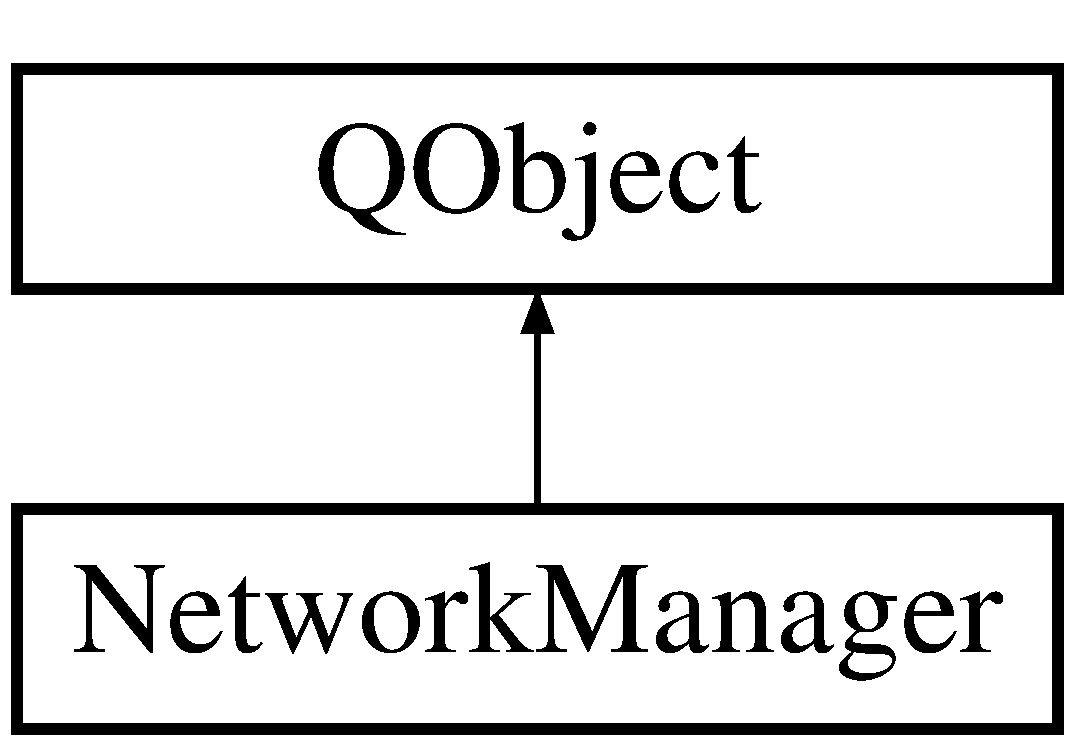
\includegraphics[height=2.000000cm]{class_network_manager}
\end{center}
\end{figure}
\subsection*{Public Member Functions}
\begin{DoxyCompactItemize}
\item 
\hyperlink{class_network_manager_afdab2fd0ea156e42ef6936caa24e4602}{Network\+Manager} (Q\+Object $\ast$parent=0)
\begin{DoxyCompactList}\small\item\em \hyperlink{class_network_manager}{Network\+Manager} Class Constructor -\/ Initializes a \hyperlink{class_network_manager}{Network\+Manager} object. \end{DoxyCompactList}\item 
Q\+\_\+\+I\+N\+V\+O\+K\+A\+B\+LE void \hyperlink{class_network_manager_ac18e89037f60537fb2c32040a9720e07}{load\+Web\+Page} (Q\+Line\+Series $\ast$open, Q\+Line\+Series $\ast$high, Q\+Line\+Series $\ast$low, Q\+String)
\begin{DoxyCompactList}\small\item\em load\+Web\+Page gets the J\+Son format data of the stock from the \href{https://www.alphavantage.co,}{\tt https\+://www.\+alphavantage.\+co,} do all the processing and plot on the graph \end{DoxyCompactList}\end{DoxyCompactItemize}


\subsection{Constructor \& Destructor Documentation}
\mbox{\Hypertarget{class_network_manager_afdab2fd0ea156e42ef6936caa24e4602}\label{class_network_manager_afdab2fd0ea156e42ef6936caa24e4602}} 
\index{Network\+Manager@{Network\+Manager}!Network\+Manager@{Network\+Manager}}
\index{Network\+Manager@{Network\+Manager}!Network\+Manager@{Network\+Manager}}
\subsubsection{\texorpdfstring{Network\+Manager()}{NetworkManager()}}
{\footnotesize\ttfamily Network\+Manager\+::\+Network\+Manager (\begin{DoxyParamCaption}\item[{Q\+Object $\ast$}]{parent = {\ttfamily 0} }\end{DoxyParamCaption})\hspace{0.3cm}{\ttfamily [explicit]}}



\hyperlink{class_network_manager}{Network\+Manager} Class Constructor -\/ Initializes a \hyperlink{class_network_manager}{Network\+Manager} object. 


\begin{DoxyParams}{Parameters}
{\em parent} & Q\+Object \\
\hline
\end{DoxyParams}


\subsection{Member Function Documentation}
\mbox{\Hypertarget{class_network_manager_ac18e89037f60537fb2c32040a9720e07}\label{class_network_manager_ac18e89037f60537fb2c32040a9720e07}} 
\index{Network\+Manager@{Network\+Manager}!load\+Web\+Page@{load\+Web\+Page}}
\index{load\+Web\+Page@{load\+Web\+Page}!Network\+Manager@{Network\+Manager}}
\subsubsection{\texorpdfstring{load\+Web\+Page()}{loadWebPage()}}
{\footnotesize\ttfamily void Network\+Manager\+::load\+Web\+Page (\begin{DoxyParamCaption}\item[{Q\+Line\+Series $\ast$}]{open,  }\item[{Q\+Line\+Series $\ast$}]{high,  }\item[{Q\+Line\+Series $\ast$}]{low,  }\item[{Q\+String}]{symbol }\end{DoxyParamCaption})}



load\+Web\+Page gets the J\+Son format data of the stock from the \href{https://www.alphavantage.co,}{\tt https\+://www.\+alphavantage.\+co,} do all the processing and plot on the graph 


\begin{DoxyParams}{Parameters}
{\em Open} & data, High Data, low data and symbol \\
\hline
\end{DoxyParams}


The documentation for this class was generated from the following files\+:\begin{DoxyCompactItemize}
\item 
networkmanager.\+h\item 
networkmanager.\+cpp\end{DoxyCompactItemize}

%--- End generated contents ---

% Index
\backmatter
\newpage
\phantomsection
\clearemptydoublepage
\addcontentsline{toc}{chapter}{Index}
\printindex

\end{document}
